\documentclass{article}


% if you need to pass options to natbib, use, e.g.:
%     \PassOptionsToPackage{numbers, compress}{natbib}
% before loading neurips_2024


% ready for submission
\usepackage[final]{neurips_2024}


% to compile a preprint version, e.g., for submission to arXiv, add add the
% [preprint] option:
%     \usepackage[preprint]{neurips_2024}


% to compile a camera-ready version, add the [final] option, e.g.:
%     \usepackage[final]{neurips_2024}


% to avoid loading the natbib package, add option nonatbib:
%    \usepackage[nonatbib]{neurips_2024}


\usepackage[utf8]{inputenc} % allow utf-8 input
\usepackage[T1]{fontenc}    % use 8-bit T1 fonts
\usepackage{hyperref}       % hyperlinks
\usepackage{url}            % simple URL typesetting
\usepackage{booktabs}       % professional-quality tables
\usepackage{amsfonts}       % blackboard math symbols
\usepackage{nicefrac}       % compact symbols for 1/2, etc.
\usepackage{microtype}      % microtypography
\usepackage{xcolor}         % colors
\usepackage{bm}
\usepackage{graphicx}
\usepackage[linesnumbered,ruled,vlined]{algorithm2e}
\usepackage{amsmath}
\usepackage{tikz}
\usepackage{float}
\usepackage{enumitem}
\usepackage{amssymb}
\newtheorem{theorem}{Theorem}[section]
\newtheorem{example}[theorem]{Example}
\newtheorem{lemma}{Lemma}
\newcommand*{\qed}{\null\nobreak\hfill\ensuremath{\square}}%



\DeclareMathOperator*{\argmax}{arg\,max}

\title{First-Order Methods in Online Convex Optimization}


% The \author macro works with any number of authors. There are two commands
% used to separate the names and addresses of multiple authors: \And and \AND.
%
% Using \And between authors leaves it to LaTeX to determine where to break the
% lines. Using \AND forces a line break at that point. So, if LaTeX puts 3 of 4
% authors names on the first line, and the last on the second line, try using
% \AND instead of \And before the third author name.


\author{%
  WONG, Hok Fong \quad LAM, Sze Yin\\
  Department of Computer Science and Engineering\\
  The Chinese University of Hong Kong\\
  \texttt{\{silaswhf, 1155193130\}@link.cuhk.edu.hk} \\
  % examples of more authors
}


\begin{document}
\IncMargin{1.5em}

\maketitle


\begin{abstract}
  Online convex optimization deals with making sequential decisions in an uncertain environment where data arrives in a streaming fashion.
  Hence, it is necessary, and beneficial, to take a robust approach, by applying an optimization method that learns as more aspects of the problem are observed.
  This view of optimization as a process has led to successes in developing efficient algorithms for prominent online learning problems.
  In this report, we present the key concepts in online convex optimization, several classic first-order online convex optimization algorithms that are robust to adversarial attacks, and showcase the applicability of the framework to the online email classification task.
\end{abstract}


\section{The Online Convex Optimization (OCO) Framework}

Online convex optimization considers optimization as a process [1], where at round $t$ the online optimizer chooses a vector $\textbf{w}_t$ from a convex decision set $\mathcal{S}\subseteq \mathbb{R}^n$ in the Euclidean space.
After the optimizer has committed to a choice, a convex cost function $f_t\in \mathcal{F}: \mathcal{S}\mapsto \mathbb{R}$ is revealed, which is picked from a bounded family of cost functions by the adversary.
The optimizer then suffer a loss of $f_t(\textbf{w}_t)$, which is undesired. We summarize the process of online convex optimization as the following [2].

\SetAlgorithmName{Model}{Model}{Model}

\begin{algorithm}[H]
  \caption{Online Convex Optimization}
  \For{$t=1,2,\ldots,T$}{
    Predict a vector $\textbf{w}_t\in \mathcal{S}$

    Receive a convex loss function $f_t: \mathcal{S}\to \mathbb{R}$

    Suffer loss $f_t(\textbf{w}_t)$
  }
\end{algorithm}

\SetAlgorithmName{Algorithm}{Algorithm}{Algorithm}

The ultimate goal of the optimizer is to minimize the cumulative sum of the losses suffered along its run. However, given that the adversary's behaviour is adaptive in nature, we have to define another fair metric called the ``regret'', by benchmarking a strategy with respect to the optimal one.
To be precise, the regret incurred by a sequence of $t$ decisions $\textbf{w}_1, \textbf{w}_2, \ldots, \textbf{w}_T\in\mathcal{S}$ given the revealed loss functions $f_1, f_2, \ldots, f_T$, is defined as \[\sum\limits_{i=1}^T f_t(\textbf{w}_t)-\min\limits_{\textbf{w}\in\mathcal{S}} \sum\limits_{i=1}^T f_t(\textbf{w}),\] which is the difference between the loss accumulated and the minimum loss that could have been accumulated.
Therefore, we restate the optimizer's goal as having the lowest possible regret relative to a hypothesis class $\mathcal{H}$ which is \[\text{Regret}_T(\mathcal{H})=\max_{h^\star \in\mathcal{H}} \text{Regret}_T(h^\star).\]
We also consider that an algorithm is learning if its regret is sublinear in $T$, i.e. $\text{Regret}_T(\mathcal{H})=o(T)$, implying that the regret per round asymptotically converges to zero as $T$ tends to infinity.

Clearly, without any additional assumptions, no algorithm can achieve low regret at all as there is no correlation between past and present rounds.
This impossibility result is attributed to Cover.
Thus, several restrictions are necessary for this framework:
\begin{enumerate}[label=\textbf{\textit{Ass.} \arabic*}:]
  \item The losses determined by an adversary should not be allowed to be unbounded. Otherwise, the adversary could keep decreasing the scale of the loss at each step, and never allow  the algorithm to recover from the loss of the first step. Thus, we assume that the losses lie in some bounded region.
  \item The decision set must be bounded and/or structured, though not necessary finite. Otherwise, the adversary can assign high loss to all the strategies chosen by the player indefinitely, while setting apart some strategies with zero loss.
\end{enumerate}



\section{Classic Problems that Can Be Modeled via Online Convex Optimization}

Online Convex Optimization (OCO) has become a leading online learning framework due to its modeling capability and its influence on the design of efficient online learning algorithms.
In Online Learning, a model is always required to perform real-time adaptation to continuous data arrivals. This learning scheme also allows a model incrementally learn a concept and update accordingly without the need to retrain on the entire dataset, efficiently reduces memory and computational costs by processsing one data point at a time.
In this section, we describe problems that arise in online learning and study some special cases of how they could fit into the OCO framework [1].

\subsection{Online Regression / Online Classification Tasks}

Online regression or classification has many applications, such as email spam classification [3].
We consider a linear classifier using a soft-margin SVM formulation for this example in the OCO framework, where the predictor receives some features of the $t$-th email $\textbf{x}_t\in \mathbb{R}^d$ in round $t$ with the ``bag-of-words'' representation along with some additional attributes.
We also require the agent to learn a filter $\textbf{w}\in\mathbb{R}^d$, which is norm-bounded within a certain radius.
Then, the cost functions are determined by $f_t(\textbf{w})=\max\{0, 1-y_t\textbf{w}^\top\textbf{x}_t\}$, which is a convex hinge loss function measured against the groundtruth label $y_t$ in every round $t$.

As a sidenote, we used a surrogate loss function for convexification, rather than a discontinuous, non-convex $0/1$ loss $f_t(\textbf{w})=\bm{1}[\text{sign}(\langle \textbf{x}_t, \textbf{w}\rangle )\neq y_t]$, which leads to efficient and computationally-tractable techniques for finding a solution to the optimization problem.

\subsection{Expert's Advice}

For the problem of prediction with expert advice, where the decision maker has to choose among the advice of $d$ experts. Denote by $p_t\in \{1,2,\ldots, d\}$ the chosen expert, then the learner receives a vector $\textbf{y}_t\in [0,1]^d$, where $y_t[i]$ is the cost of following the advice of the $i$-th expert. The learner pays the loss $y_t[p_t]$. The decision space in this problem is discrete.

However, by allowing the learner to randomize its predictions where we let $\mathcal{S}=\{\textbf{w}\in \mathbb{R}^d: \textbf{w}\geq 0\wedge \lVert \textbf{w}\rVert_1=1\}$ be the probability simplex forming a convex set, and let the learner choose $\textbf{w}_t\in \mathcal{S}$ according to the distribution, we can restrict the power of the adversarial environment by analyzing the expected cost of the learner \[\mathbb{E}[y_t[p_t]]=\sum\limits_{i=1}^d \mathbb{P}[p_t=i]y_t[i]=\langle \textbf{w}_t, \textbf{y}_t\rangle.\]
Now, in OCO, we can set $f_t(\textbf{w})=\langle \textbf{w}, \textbf{y}_t\rangle$ and analyze the regret against the set of competiting vectors $U$, i.e. the $d$ singletons of the form $(0,\ldots, 0,1,0,\ldots, 0)$, corresponding to always following the advice of a single expert.
Note that the decision set $\mathcal{S}$ is a convex simplex, and the cost functions are linear and bounded in the $L_\infty$-norm.

\section{First-Order Online Convex Optimization Algorithms}

\subsection{Follow-the-Leader}
One primitive idea is to consider at any time the optimal vector which incurs the minimal loss on all past rounds [5]. This strategy is known as ``Follow-the-Leader'' (FTL) in machine learning [2, 3].

\begin{algorithm}[H]
  \caption{Follow-The-Leader Algorithm (Kalai and Vempala, 2005)}
  \For{$i=1,2,\ldots, T$}{
    Predict a vector $\textbf{w}_i=\arg\min_{\textbf{w}\in \mathcal{S}} \sum_{t=1}^{i-1} f_i(\textbf{w})$

    Receive a convex loss function $f_i: \mathcal{S}\to \mathbb{R}$ and suffer loss $f_i(\textbf{w}_i)$
  }
\end{algorithm}

Although Theorem 3.1 shows a success of FTL for a sub-family of online convex optimization, FTL could fail in a worse-case scenario even for the linear optimization problem, shown in Example 3.2 [2, 3].

\begin{theorem}[Regret of FTL on Online Quadratic Optimization]
  Consider the online optimization problem where at each round $f_t(\textbf{w})=\frac{1}{2}\lVert \textbf{w}-\textbf{z}_t\rVert_2^2$ for some vector $\textbf{z}_t$. Then, running FTL on the problem with $\mathcal{S}=\mathbb{R}^d$ and let $L=\max_t\lVert \textbf{z}_t\rVert_2$. The regret of FTL with respect to all vectors $\textbf{u}\in \mathbb{R}^d$ is at most $4L^2(\log(T)+1)$.
\end{theorem}

\begin{example}[Failure of FTL]
  Let $\mathcal{S}=[-1,+1]$ and conider the sequence of losses $f_t(w)=z_t w$ where \[z_t=\begin{cases}-0.5, &\text{if }t=1\\1, &\text{if }t\text{ is even}\\-1, &\text{if }t>1 \wedge t\text{ is odd}\end{cases}\] Then, the predictions of FTL is set to $w_t=1$ for $t$ odd and $w_t=-1$ for $t$ even. Then, the cumulative loss and regret will both be $T$ as the fixed solution $u=0\in \mathcal{S}$ has cumulative loss 0.
\end{example}

We observed that FTL fails in Example 3.2 because of its unstable predictions, $\textbf{w}_t$ shifts drastically from round to round where we only added a single loss function to the objective of the optimization problem in the definition of $\textbf{w}_t$. This is shown in Figure 3 in Appendix A. In contrast, FTL works fine for the quadratic problem since the gradient is Lipschitz, making $\textbf{w}_{t+1}$ close to $\textbf{w}_t$.

\subsection{Follow-the-Regularized-Leader}

To stablize FTL, one way is to add a regularization term. Specifically, we consider regularizers that are strongly-convex over $\mathcal{S}$, yielding the FTRL algorithm below [2, 4].

\begin{algorithm}[H]
  \caption{Follow-The-Regularized-Leader Algorithm (Shalev-Shwartz, 2007)}
  \For{$i=1,2,\ldots, T$}{
    Predict a vector $\textbf{w}_i=\arg\min_{\textbf{w}\in \mathcal{S}} \sum_{t=1}^{i-1} f_i(\textbf{w})+R(\textbf{w})$

    Receive a convex loss function $f_i: \mathcal{S}\to \mathbb{R}$ and suffer loss $f_i(\textbf{w}_i)$
  }
\end{algorithm}

Based on Theorem 3.3, we have an $O(\sqrt{T})$ regret bound for a general family of convex functions. The case for the online linear optimization problem is shown in Example 3.4.

\begin{theorem}[Regret of FTRL]
  Let $f_1, f_2, \ldots, f_T$ be a sequence of convex functions such that $f_t$ is $L_t$-Lipschitz with respect to some norm $\lVert \cdot \rVert$.
  Let $L$ be such that $\frac{1}{T}\sum_{t=1}^T L_t^2\leq L^2$.
  Then, running FTRL on the sequence with a $\sigma$-strongly-convex regularization function with respect to the same norm.
  For all $\textbf{u}\in \mathcal{S}$, $\text{Regret}_T(\textbf{u})\leq R(\textbf{u})-\min_{\textbf{v}\in \mathcal{S}} R(\textbf{v})+TL^2/\sigma$.
  Specifically, if $U=\{\textbf{u}:\lVert \textbf{u}\rVert_2\leq B\}$ and $\eta=\frac{B}{L\sqrt{2T}}$ then $\text{Regret}_T(U)\leq BL\sqrt{2T}$.
\end{theorem}

\begin{example}[Regret of FTRL on Online Linear Optimization]
  Consider FTRL on the sequence of losses $f_t(\textbf{w})=\langle \textbf{w}, \textbf{z}_t\rangle$ and let $\mathcal{S}=\mathbb{R}^d, U=\{\textbf{u}:\lVert \textbf{u}\rVert_2\leq B\}$, $R(\textbf{w})=\frac{1}{2\eta}\lVert \textbf{w}\rVert_2^2$ where $\eta=\frac{B}{L\sqrt{2T}}>0$. Then, $\textbf{w}_{t+1}=-\eta \sum_{i=1}^t \textbf{z}_i$, and $\text{Regret}_T(\textbf{u})\leq R(\textbf{u})+TL^2\eta=\frac{1}{2\eta}\lVert\textbf{u}\rVert_2^2+TL^2\frac{B}{L\sqrt{2T}}\leq \frac{BL\sqrt{2T}}{2}+TL\frac{B\sqrt{2T}}{2T}=BL\sqrt{2T}$ for all $\textbf{u}\in \mathcal{S}$.
\end{example}
\subsection{Online Gradient Descent}

Inspired by standard gradient descent from offline optimization, the simplest algorithm that applies to the most general setting of online convex optimization is online gradient descent (OGD) [6].

\begin{algorithm}[H]
  \caption{Online Gradient Descent Algorithm (Zinkevich, 2003)}
  Initialize and predict using the vector $\textbf{w}_1=\textbf{0}$

  \For{$i=2,\ldots, T$}{
    Predict a vector $\textbf{w}_i=\textbf{w}_{i-1}-\eta\textbf{z}_{t-1}$, where $\textbf{z}_{t-1}\in \partial f_{t-1}(\textbf{w}_{t-1})$

    Receive a convex loss function $f_i: \mathcal{S}\to \mathbb{R}$ and suffer loss $f_i(\textbf{w}_i)$
  }
\end{algorithm}

The analysis for OGD is summarized below in Theorem 3.5.

\begin{theorem}[Regret of OGD]
  Let $f_1, f_2, \ldots, f_T$ be a sequence of convex functions such that $f_t$ is $L_t$-Lipschitz with respect to some norm $\lVert \cdot \rVert$.
  Let $L$ be such that $\frac{1}{T}\sum_{t=1}^T L_t^2\leq L^2$.
  Then, the regret of OGD satisfies $\text{Regret}_T(\textbf{u})\leq \frac{1}{2\eta}\lVert \textbf{u}\rVert_2^2+\eta TL^2$, for all $\textbf{u}\in \mathcal{S}$.
  Specifically, if $U=\{\textbf{u}:\lVert \textbf{u}\rVert_2\leq B\}$ and $\eta=\frac{B}{L\sqrt{2T}}$ then $\text{Regret}_T(U)\leq BL\sqrt{2T}$.
\end{theorem}

\subsection{Online Mirror Descent}

In this subsection, we derive and analyze the family of Online Mirror Descent (OMD) algorithms from the FTRL framework. Compared to FTRL, OMD has a much simpler update step, but it achieves the same regret bound as FTRL.

The starting point for OMD is to apply FTRL on a sequence of linear functions [7]. Then, assuming that $R(\textbf{w})=\infty$ for $\textbf{w}\notin \mathcal{S}$ and the notation $\textbf{z}_{1:t}=\sum_{i=1}^t \textbf{z}_i$, the prediction of FTRL can be written as follows: \[\textbf{w}_{t+1}=\arg\min_{\textbf{w}}R(\textbf{w})+\langle \textbf{w}, \textbf{z}_{1:t}\rangle=\arg\max_{\textbf{w}} \langle \textbf{w}, -\textbf{z}_{1:t}\rangle-R(\textbf{w}).\]
Rewriting $g(\bm{\theta})=\arg\max_{\textbf{w}} \langle \textbf{w},\bm{\theta}\rangle-R(\textbf{w})$, we have the two-step update rule:  $$\bm{\theta}_{t+1}=\bm{\theta}_t-\textbf{z}_t$$ $$\textbf{w}_{t+1}=g(\bm{\theta}_{t+1})$$

Now, if $f_t$ is convex but nonlinear, then we can use subgradients of $f_t$ at $\textbf{w}_t$ to linearize the problem, so that $f_t(\textbf{w}_t)-f_t(\textbf{u})\leq \langle \textbf{w}_t, \textbf{z}_t\rangle-\langle \textbf{u}, \textbf{z}_t\rangle$; hence, the regret with respect to the nonlinear loss functions is upper bounded by the regret with respect to the linear functions, yielding the OMD framework below [7].

\begin{algorithm}[H]
  \caption{Online Mirror Descent Algorithm (Hazan and Kale, 2008)}
  Initialize $\bm{\theta}_1=\textbf{0}$

  \For{$i=1,\ldots, T$}{
    Predict a vector $\textbf{w}_i=g(\bm{\theta}_t)$

    Update $\bm{\theta}_{t+1}=\bm{\theta}_t-\textbf{z}_t$ where $\textbf{z}_t\in \partial f_t(\textbf{w}_t)$

    Receive a convex loss function $f_i: \mathcal{S}\to \mathbb{R}$ and suffer loss $f_i(\textbf{w}_i)$
  }
\end{algorithm}

It is also clear that OGD is a special case of OMD, where $\mathcal{S}=\mathbb{R}^d$ and $g(\bm{\theta})=\eta\bm{\theta}$ for some $\eta>0$. For the general case where $g$ is non-linear, the update of $\bm{\theta}$ is being carried out in a ``dual'' space by subtracting the gradient out of it, and the actual prediction is mirrored to the set $\mathcal{S}$ via the function $g$. The choice of the regularizer forms a sense of duality: transforming the space of gradient updates, from $\mathbb{R}^n$ onto itself. This is summarized in Figure 1.

\begin{figure}[H]
  \centering
  \includegraphics[width=0.5\linewidth]{../../mirror.png}
  \caption{OMD update in terms of duality mappings, where $\nabla \psi$ is the mirror map and $(\nabla \psi)^{-1}$ is the inverse of the mirror map.}
\end{figure}

We provide a generic bound for the OMD family of algorithms based on the analysis of the FTRL algorithm, concluded by Theorem 3.6.

\begin{theorem}
  Let $R$ be a $(1/\eta)$-strongly-convex function over $\mathcal{S}$ with respect to a norm $\lVert \cdot\rVert$. Assume that OMD is run on the sequence with a link function $g(\bm{\theta})=\arg\max_{\textbf{w}\in \mathcal{S}} (\langle \textbf{w},\bm{\theta}\rangle-R(\textbf{w}))$. Then, for all $\textbf{u}\in \mathcal{S}$, $\text{Regret}_T(\textbf{u})\leq R(\textbf{u})-\min_{\textbf{v}\in \mathcal{S}} R(\textbf{v})+\eta\sum_{t=1}^T \lVert \textbf{z}_t\rVert_\star ^2$, where $\lVert \cdot\rVert_\star$ is the dual norm. Furthermore, if $f_t$ is $L_t$-Lipschitz with respect to $\lVert\cdot\rVert$, then $\lVert \textbf{z}_t\rVert_\star\leq L_t$.
\end{theorem}


\subsection{The Doubling Trick}

For the algorithms demonstrated earlier, the parameter $\eta$ depends on the time horizon $T$, which should be avoided in real applications. However, the doubling trick enables us to convert such an algorithm requiring the knowledge of $T$ into one without the knowledge that enjoys the same (asymptotic) regret bound.
The fundamental idea is to divide the time into periods of increasing size and run the original algorithm on each period [2].

\begin{algorithm}[H]
  \caption{The Doubling Trick}
  \For{$i=0,1,2,\ldots$}{
    Run the algorithm $\mathcal{A}$ on the $2^m$ rounds $t=2^m, \ldots, 2^{m+1}-1$.
  }
\end{algorithm}

To see that the converted algorithm indeed achieves the bound, note that the regret of $\mathcal{A}$ on each period of $2^m$ rounds is at most $\alpha \sqrt{2^m}$. Therefore, the total regret is at most \[\sum\limits_{i=1}^{\lceil\log_2 T\rceil}\alpha\sqrt{2^m}=\alpha\sum\limits_{i=1}^{\lceil \log_2 T\rceil} (\sqrt{2})^m=\alpha\frac{1-\sqrt{2}^{\lceil \log_2 T\rceil +1}}{1-\sqrt{2}}\leq \alpha\frac{1-\sqrt{2T}}{1-\sqrt{2}}\leq \frac{\sqrt{2}}{\sqrt{2}-1}\alpha \sqrt{T}.\]
Hence, the regret is only worse by a multiplicative factor $\frac{\sqrt{2}}{\sqrt{2}-1}$.
\section{Experiment}

\paragraph{Online Email Spam Classification} We demonstrate the potential of some algorithms in Section 3 with the email categorization task, utilizing a soft-margin linear SVM with hinge loss, as has been described in Section 2.1.

\paragraph{Dataset.} We use the \texttt{Spambase} dataset adapted from the UCI Machine Learning Repository. The dataset contains $4601$ emails, each represented by $57$ features $n=57$. We assume that the emails arrives in sequence and are classified one after the other, making $T=4601$ predictions. All the $4601$ feature vectors are normalized with an $L_2$-norm of $1$.

\paragraph{Algorithms and Settings.} We train a model to learn a filter $\textbf{w}\in \mathbb{R}^{4601}$, using FTL, FTRL with the regularizer $R(\textbf{w})=\frac{1}{2\eta}\lVert \textbf{w}\rVert_2^2$, and OGD with the learning rate same as $\eta$. We emphasize that $\eta$ is chosen to minimize the regret bound, which is given by $$\eta=\frac{B}{L\sqrt{2T}}=\frac{2}{1\times \sqrt{2\times 4601}}=0.0208.$$

\paragraph{Result.} We display the results for the online email classification task in Table 1.

First, the regret of FTRL is similar to that of OGD, which verifies the theoretical regret bound $$\text{Regret}_T(U)\leq BL\sqrt{2T}=2\times\sqrt{2\times 4601}=191.$$

Second, we can see that the regret's growth is limited under a line (shown in Figure 2), and seems to be asymptotically sublinear.

\begin{figure}[H]
  \centering
  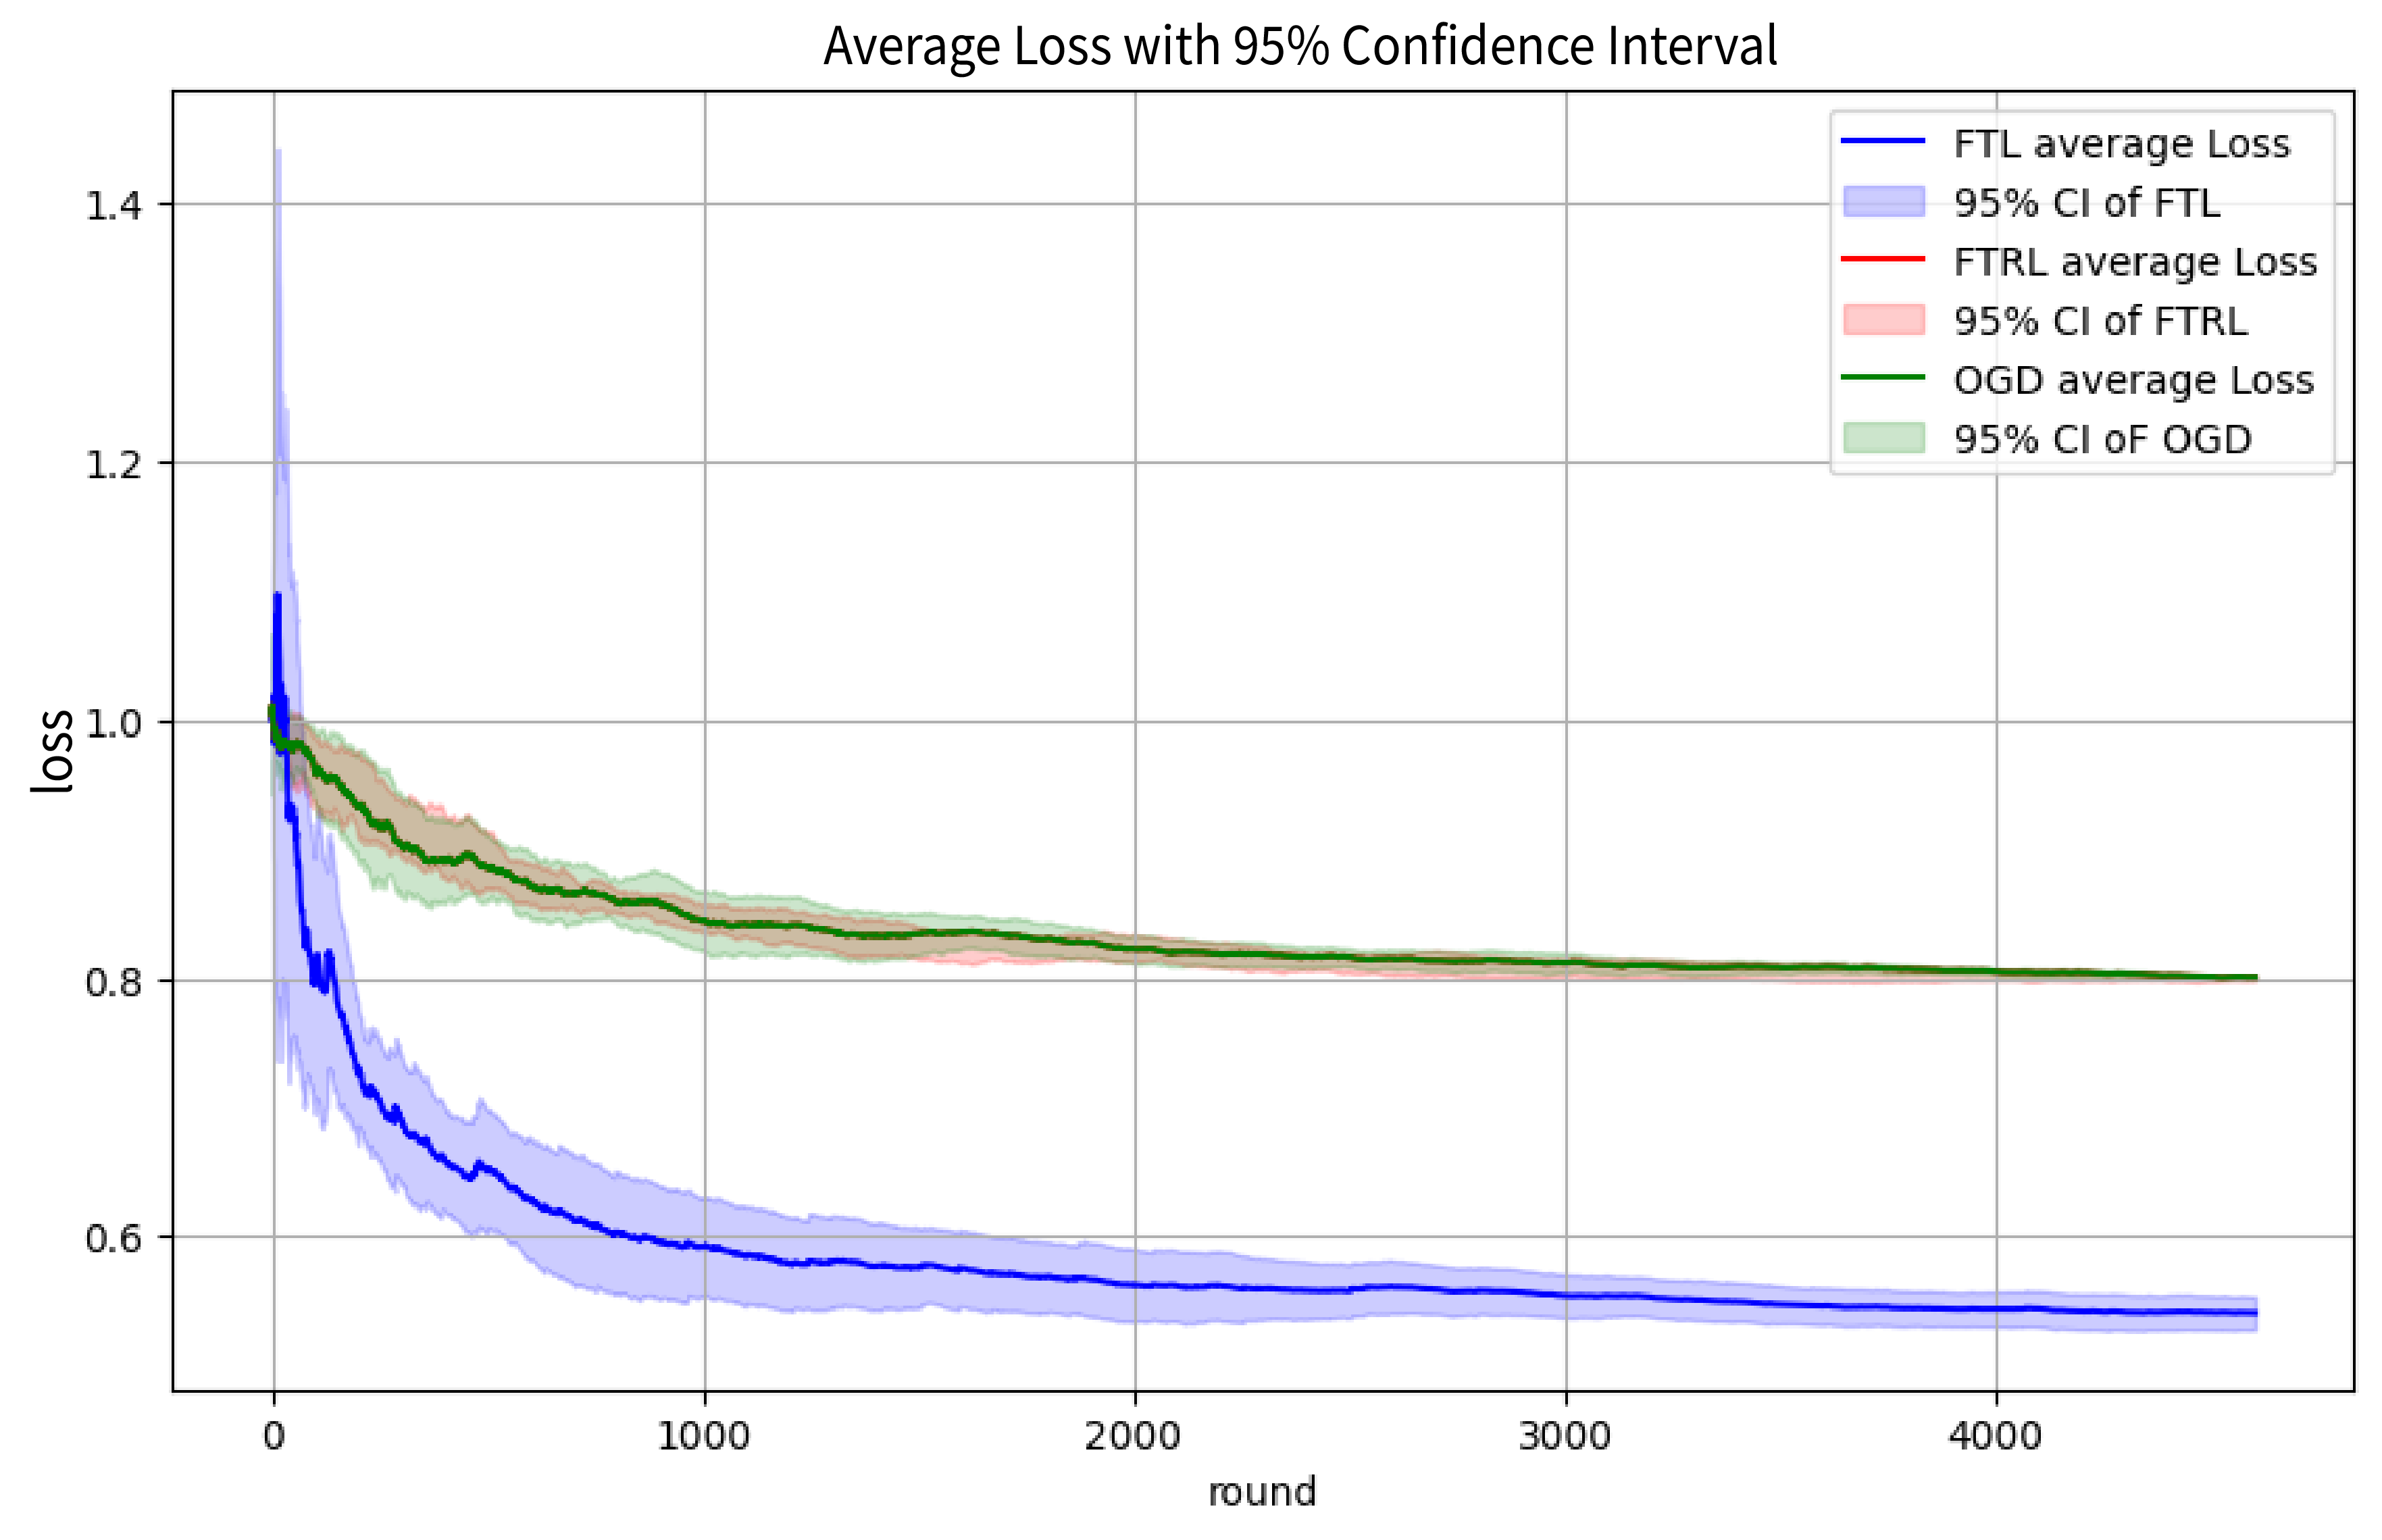
\includegraphics[width=0.48\linewidth]{../LossAvgF.png}
  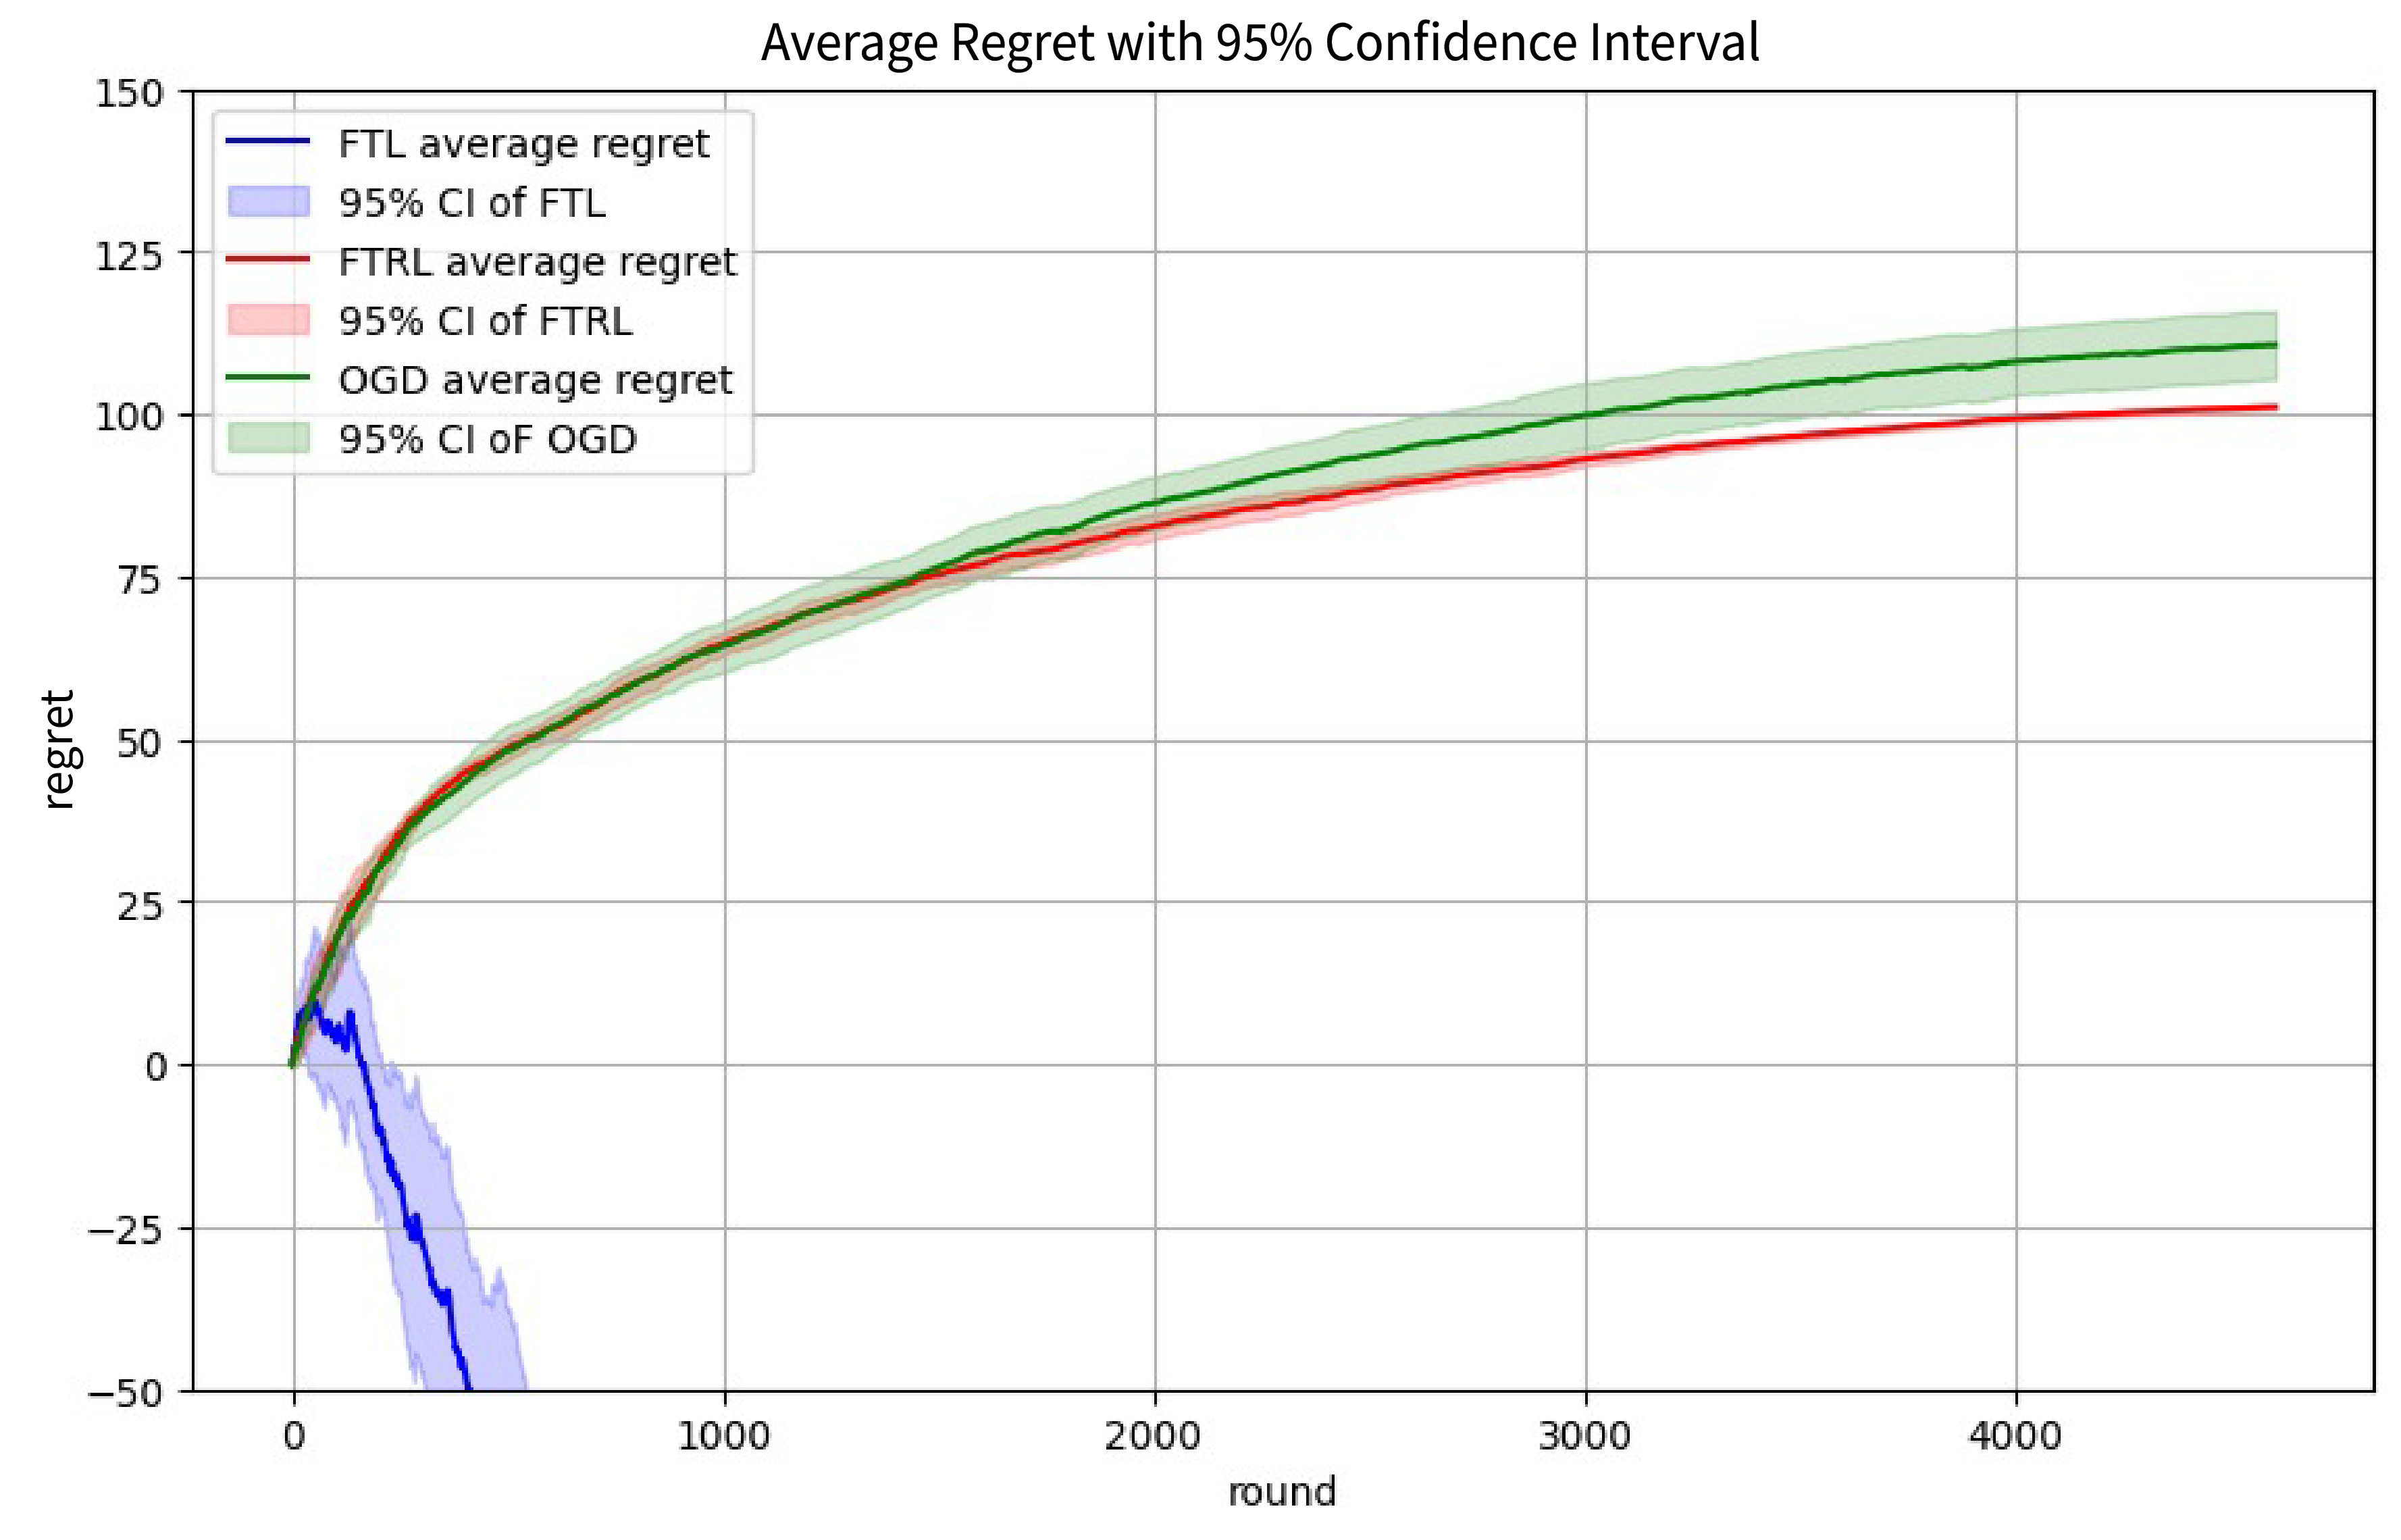
\includegraphics[width=0.48\linewidth]{../regretAvgF.png}

  \caption{Performance of various algorithms in the email classfication tasks, illustrating the averaged cumulative loss for each round (left panel) and the cumulative regret till round $t$ (right panel).}
\end{figure}

Thirdly, it is also surprising that FTL has outperformed both FTRL and OGD (see Table 1). This is due to the aggressive nature of FTL, we can see that the regret per round of FTL surged up to $1.2$, which is vulnerable to attacks. We suspect that the dataset is lenient to FTL as the algorithm tunes the model without being tricked, which helps it achieve a better result by taking larger steps for updates, and eventually, converges to the optimal point.

\begin{table}[H]
  \centering
  \caption{Main results for the email classification task (optimal vector is taken from $U$ with $B=2$, dataset shuffled for $10$ independent experiments).}

  \begin{tabular}{c c c c}
    \toprule
    \textbf{Methods}  & \textbf{FTL}        & \textbf{FTRL}      & \textbf{OGD}      \\ \midrule
    Avg. mistakes     & $1,074.20\pm37.42$  & $1,814.70\pm 3.16$ & $1,818.80\pm42.1$ \\
    Cumulative regret & $-1,122.78\pm62.53$ & $100.76\pm 0.86$   & $113.48\pm6.50$   \\
    \bottomrule
  \end{tabular}

\end{table}

\section{Summary}
In this paper, we present several first-order algorithms in online convex optimization that are feasible for the online learning settings. For each of these algorithms, we also provide theoretical guarantees on the regret bound that justifies the learnability of the algorithms. We have also demonstrated one possible application of online convex optimization on the online email spam classification task,  verifying the regret analyses.

\newpage
\section*{References}
{
\small


[1] Orabona, F.\ (2023) A Modern Introduction to Online Learning.
  {\it arXiv}. \url{https://arXiv.org/pdf/1912.13213}.

[2] Shalev-Shwartz, S.\ (2011) Online Learning and Online Convex Optimization.
  {\it Foundations and Trends in Machine Learning} {\bf 4}(2). \url{https://www.cs.huji.ac.il/~shais/papers/OLsurvey.pdf}.

[3] Hazan, E.\ (2021) Introduction to Online Convex Optimization.
  {\it arXiv}. \url{https://arxiv.org/pdf/1909.05207}.

[4] Shalev-Shwartz, S.\ (2007) {\it Online Learning and Online Learning: Theory, Algorithms, and Applications}.
Doctoral Thesis, Hebrew University. \url{https://home.ttic.edu/~shai/papers/ShalevThesis07.pdf}.

[5] Kalai, A. and Vempala, S.\ (2005) Efficient algorithms for online decision problems. {\it Journal of Computer and System Sciences} {\bf 71}(3):291-307.

[6] Zinkevich, M. \ (2003) Online convex programming and generalized infinitesimal gradient ascent. {\it Proceedings of the 20th International Conference on Machine Learning}, 928-936.

[7] Hazan, E. and Kale, S. \ (2008) Extracting certainty from uncertainty: Regret bounded by variation in costs. {\it The 21st Annual Conference on Learning Theory (COLT)}, 57-68.

}

%%%%%%%%%%%%%%%%%%%%%%%%%%%%%%%%%%%%%%%%%%%%%%%%%%%%%%%%%%%%

\appendix

\section{Failure of FTL}

Consider Example 3.2 again, let $\mathcal{S}=[-1,+1]$ and the sequence of losses $f_t(w)=z_t w$ where \[z_t=\begin{cases}-0.5, &\text{if }t=1\\1, &\text{if }t\text{ is even}\\-1, &\text{if }t>1 \wedge t\text{ is odd}\end{cases}\] Then, the predictions of FTL is set to $w_t=1$ for $t$ odd and $w_t=-1$ for $t$ even.

In Figure 3 and 4, we colored the predictions $w_t$ green, in arrows, and the scalar $z_t$ picked by the adversary which decides the loss function, as blue. While the algorithm wishes to receive $z_t$'s that lie on the other side of the $y$-axis, the adversary does the opposite by picking exactly what FTL provides, resulting in a loss of $1$ in each round.

\begin{figure}[H]
  \centering
  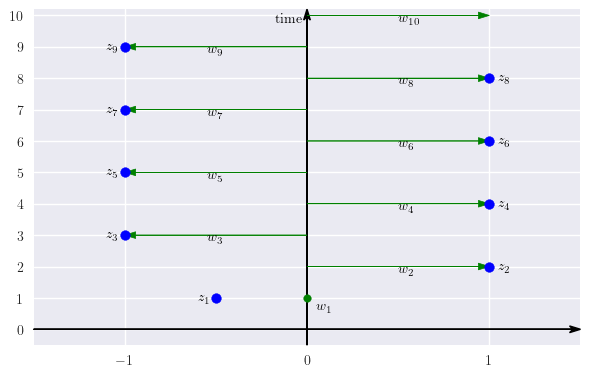
\includegraphics[width=0.5\linewidth]{../FTL_demo.png}
  \caption{Illustration of the prediction of FTL and the choice made by the adversary.}
\end{figure}

In contrast, FTRL is more conservative as the step size for the online linear optimization is only $\eta$ per update, adjusted against the adversarial environment.

\begin{figure}[H]
  \centering
  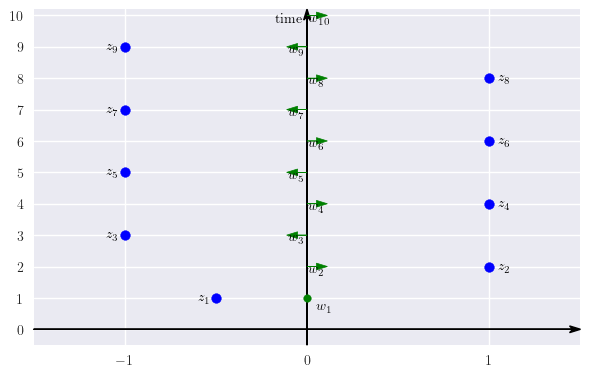
\includegraphics[width=0.5\linewidth]{../FTRL_demo.png}
  \caption{Illustration of the prediction of FTRL and the choice made by the adversary.}
\end{figure}

\section{Proof of Theorems}

\subsection{Proof of Theorem 3.1}
\begin{lemma}
  Let $\textbf{w}_1, \textbf{w}_2, \ldots$ be the sequence of vectors produced by FTL. Then, for all $\textbf{u}\in S$ we have \[\text{Regret}_T(\textbf{u})=\sum\limits_{t=1}^T (f_t(\textbf{w}_t)-f_t(\textbf{u}))\leq \sum\limits_{t=1}^T (f_t(\textbf{w}_t)-f_t(\textbf{w}_{t+1})).\]
\end{lemma}

{\it Proof.} Proof by induction. Subtracting $\sum_t f_t(\textbf{w}_t)$ from both sides of the inequality and rearranging yields $\sum_{t=1}^T f_t(\textbf{w}_{t+1})\leq \sum_{t=1}^T f_t(\textbf{u})$. The base case is direct from the definition. Assume the inequality holds for $T$, then for $T+1$ we have \[\begin{aligned}\min\limits_{\textbf{u}\in\mathcal{S}}\sum\limits_{t=1}^{T+1} f_t(\textbf{u})=\sum\limits_{t=1}^{T+1} f_t(\textbf{w}_{T+2})&\overset{\text{by }{\it def.}}{\geq} &&\sum\limits_{t=1}^T f_t(\textbf{w}_{T+1})+f_{T+1}(\textbf{w}_{T+2})\\&\overset{\text{by IH}}{\geq} &&\sum\limits_{t=1}^T f_t(\textbf{w}_{t+1})+f_{T+1}(\textbf{w}_{T+2})=\sum\limits_{t=1}^{T+1} f_t(\textbf{w}_{t+1}).\end{aligned}\]\qed

{\it Proof of Theorem 3.1.} It is easy to verify that $\textbf{w}_t=\frac{1}{t-1}\sum_{i=1}^{t-1} \textbf{z}_i$.
We can also rewrite $\textbf{w}_{t+1}=\frac{1}{t}(\textbf{z}_t+(t-1)\textbf{w}_t)=(1-1/t)\textbf{w}_t+1/t\cdot\textbf{z}_t$, which yields $\textbf{w}_{t+1}-\textbf{z}_t=(1-1/t)(\textbf{w}_t-\textbf{z}_t)$.
Therefore, \[f_t(\textbf{w}_t)-f_t(\textbf{w}_{t+1})=\frac{1}{2}\lVert \textbf{w}_t-\textbf{z}_t\rVert^2_2-\frac{1}{2}\lVert \textbf{w}_{t+1}-\textbf{z}_t\rVert_2^2=\frac{1}{2}\left(1-\left(1-1/t\right)^2\right)\lVert\textbf{w}_t-\textbf{z}_t\rVert_2^2\leq \frac{1}{2}\lVert \textbf{w}_t-\textbf{z}_t\rVert_2^2.\]
Since $\textbf{w}_t$ is the average of $\textbf{z}_1, \ldots, \textbf{z}_{t-1}$ we have $\lVert \textbf{w}_t\rVert_2\leq L$ and therefore, $\lVert \textbf{w}_t-\textbf{z}_t\rVert\leq 2L.$
Hence, \[\sum\limits_{t=1}^T (f_t(\textbf{w}_t)-f_t(\textbf{w}_{t+1}))\leq (2L)^2 \sum\limits_{t=1}^T \frac{1}{t}\leq 4L^2(\log T+1).\]\qed

\subsection{Proof of Theorem 3.3}
{\it Proof of Theorem 3.3.} Observe that running FTRL on $f_1, \ldots, f_T$ is equivalent to running FTL on $f_0, f_1, \ldots, f_T$ where $f_0=R$. Using Lemma 1, we obtain \[\sum\limits_{t=0}^T (f_t(\textbf{w}_t)-f_t(\textbf{u}))\leq \sum\limits_{t=0}^T (f_t(\textbf{w}_t)-f_t(\textbf{w}_{t+1})).\] Rearranging and use $f_0=R$, we now have \[\text{Regret}_T (\textbf{u})\leq R(\textbf{u})-R(\textbf{w}_1)+\sum\limits_{t=1}^T (f_t(\textbf{w}_t)-f_t(\textbf{w}_{t+1}))\leq R(\textbf{u})-\min\limits_{\textbf{v}\in\mathcal{S}}R(\textbf{v})+\sum\limits_{t=1}^T (f_t(\textbf{w}_t)-f_t(\textbf{w}_{t+1})).\] Since $f_t$ is $L_t$-Lipschitz with respect to a norm, $f_t(\textbf{w}_t)-f_t(\textbf{w}_{t+1})\leq L\lVert \textbf{w}_t-\textbf{w}_{t+1}\rVert$. By strong-convexity of $R$, we consider $F_t(\textbf{w})=\sum_{i=1}^{t-1}f_i(\textbf{w})+R(\textbf{w})$ which is also $\sigma$-strongly-convex, and note that $\textbf{w}_t=\arg\min_{\textbf{w}\in \mathcal{S}}F_t(\textbf{w}).$ This implies \[F_t(\textbf{w}_{t+1})\geq F_t(\textbf{w}_t)+\frac{\sigma}{2}\lVert \textbf{w}_t-\textbf{w}_{t+1}\rVert^2.\] Repeating the same argument for $F_{t+1}$ and its minimizer $\textbf{w}_{t+1}$ yields \[F_{t+1}(\textbf{w}_{t})\geq F_{t+1}(\textbf{w}_{t+1})+\frac{\sigma}{2}\lVert \textbf{w}_t-\textbf{w}_{t+1}\rVert^2.\] Hence, summing up the two inequalities we have \[\sigma \lVert \textbf{w}_t-\textbf{w}_{t+1}\rVert^2\leq f_t(\textbf{w}_t)-f_t(\textbf{w}_{t+1})\leq L_t\lVert \textbf{w}_t-\textbf{w}_{t+1}\rVert.\] Rearranging, we obtain $\lVert \textbf{w}_t-\textbf{w}_{t+1}\rVert\leq L_t/\sigma$, which concludes the proof.\qed

\subsection{Proof of Theorem 3.5}
{\it Proof of Theorem 3.5.} In each round $t$, there exists a subgradient $\textbf{z}_t$ such that for all $\textbf{u}$, $f_t(\textbf{w}_t)-f_t(\textbf{u})\leq \langle \textbf{w}_t-\textbf{u}, \textbf{z}_t\rangle$.
Hence, \[\sum\limits_{t=1}^T (f_t(\textbf{w}_t)-f_t(\textbf{u}))\leq \sum\limits_{t=1}^T (\langle \textbf{w}_t, \textbf{z}_t\rangle-\langle \textbf{u}, \textbf{z}_t\rangle).\]
Also, \[\begin{aligned}\text{Regret}_T(\textbf{u})&\leq R(\textbf{u})-R(\textbf{w}_1)+\sum\limits_{t=1}^T (f_t(\textbf{w}_t)-f_t(\textbf{w}_{t+1}))\\&\leq \frac{1}{2\eta}\lVert \textbf{u}\rVert_2^2+\sum\limits_{t=1}^T\langle \textbf{w}_t-\textbf{w}_{t+1}, \textbf{z}_t\rangle=\frac{1}{2\eta}\lVert \textbf{u}\rVert_2^2+\eta \sum\limits_{t=1}^T\lVert \textbf{z}_t\rVert_2^2.\end{aligned}\] Since $f_t$ is Lipschitz, the term $\sum_{t=1}^T \lVert \textbf{z}_t\rVert_2^2$ can be bounded by $\sum_{t=1}^T L_t^2\leq L$, concluding the proof.\\\qed


\subsection{Proof of Theorem 3.6}
{\it Proof of Theorem 3.6.} As shown previously, $f_t(\textbf{w}_t)-f_t(\textbf{u})\leq \langle \textbf{w}_t-\textbf{u}, \textbf{z}_t\rangle$. Since OMD is equivalent to running FTRL on the sequence of linear functions with the regularization $R(\textbf{w})$, it immediately follows the theorem.\qed

\end{document}